% Figure 1 -- software architecture of edikit: modules, data flow, entry
% points, and which components stop execution versus record a finding.
% Single source: the manuscript includes the PDF built from this file, and
% the same PDF is the separate figure upload. Build reproducibly with
%   SOURCE_DATE_EPOCH=0 FORCE_SOURCE_DATE=1 latexmk -pdf figure1.tex
\documentclass[tikz,border=6pt]{standalone}
\usetikzlibrary{positioning,arrows.meta,fit,backgrounds,calc}
\begin{document}
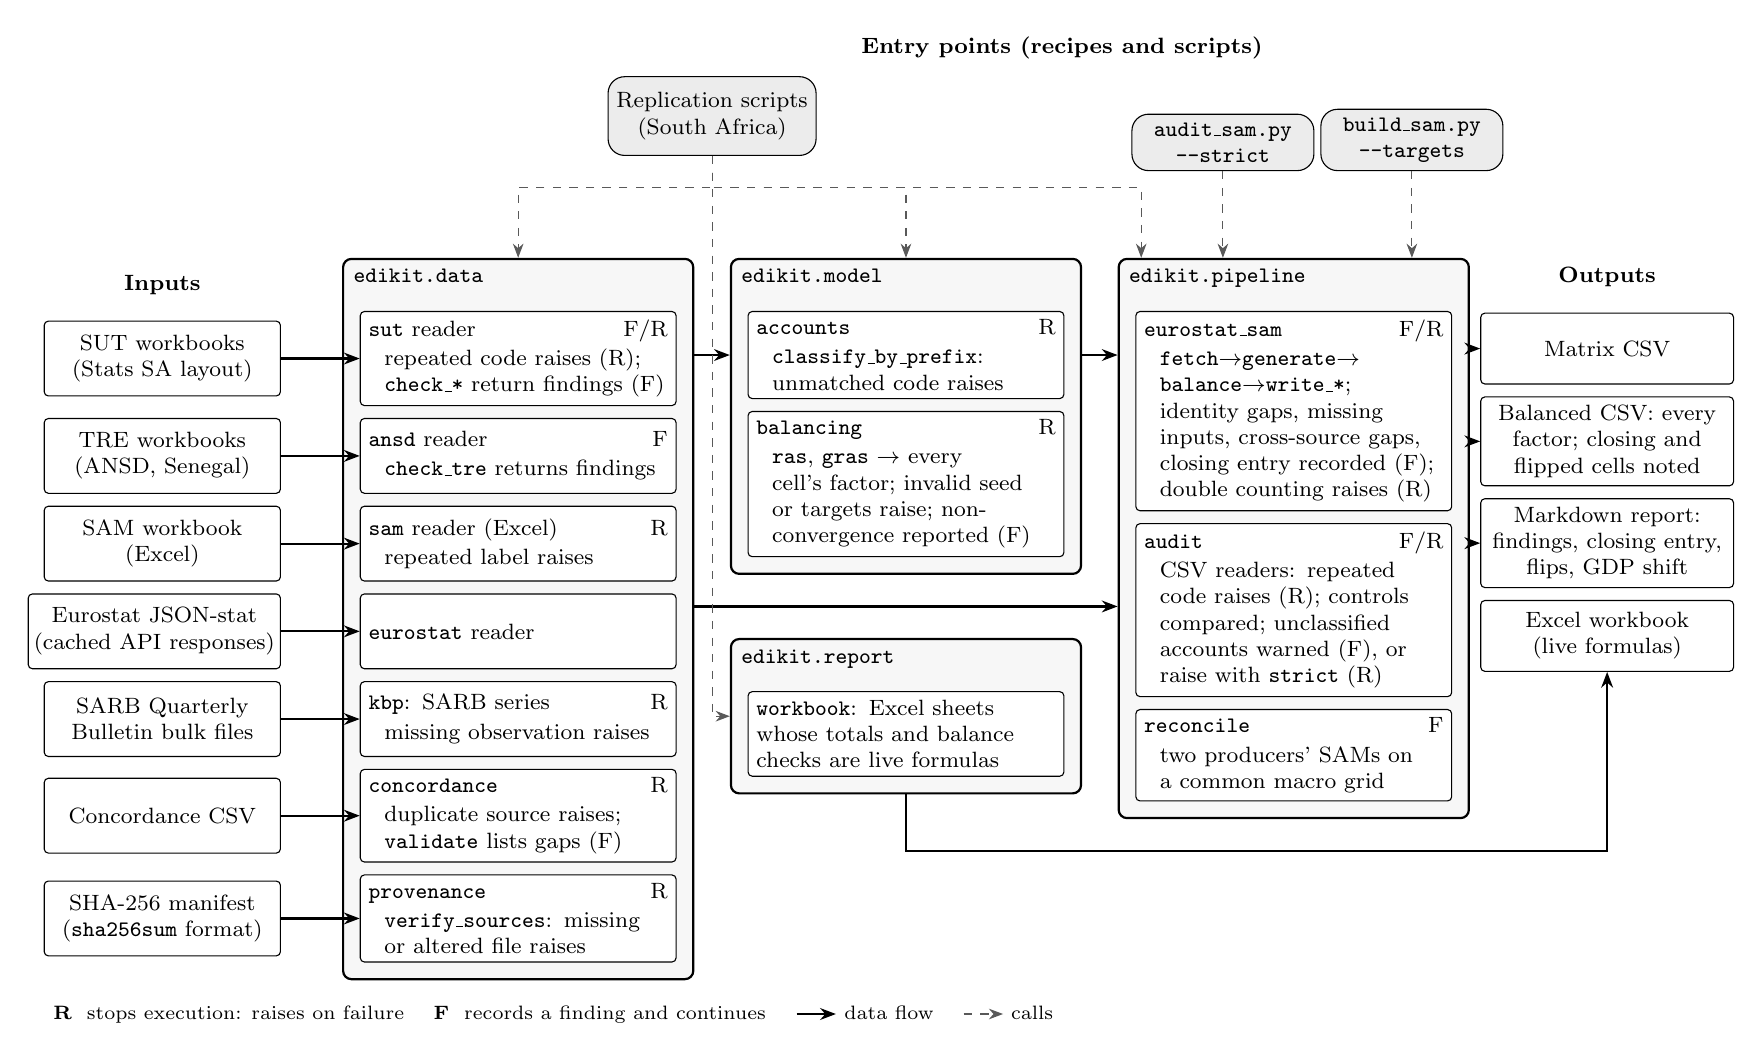
\begin{tikzpicture}[
  font=\footnotesize,
  inbox/.style={draw, rounded corners=1.5pt, align=center, fill=white,
                minimum width=30mm, minimum height=9.5mm, inner sep=2pt},
  comp/.style={draw, rounded corners=1.5pt, align=left, fill=white,
               text width=38mm, inner sep=3pt, minimum height=9.5mm},
  outbox/.style={draw, rounded corners=1.5pt, align=center, fill=white,
                 text width=30mm, inner sep=3pt, minimum height=9mm},
  entry/.style={draw, rounded corners=6pt, align=center, fill=gray!15,
                minimum height=7mm, inner sep=3pt},
  pkg/.style={draw, thick, rounded corners=3pt, fill=gray!6, inner sep=6pt},
  title/.style={font=\footnotesize\bfseries, anchor=north west, inner sep=4pt},
  head/.style={font=\footnotesize\bfseries},
  flow/.style={-{Stealth[length=2mm]}, thick},
  call/.style={-{Stealth[length=1.8mm]}, dashed, gray!70!black},
  R/.style={font=\scriptsize\bfseries},
]

% ---------- edikit.data: one reader per input, so every arrow is straight ----------
\node[comp] (d1) at (0,0)
  {\texttt{sut} reader \hfill F/R\\[1pt]
   \hspace*{2mm}repeated code raises (R);\\
   \hspace*{2mm}\texttt{check\_*} return findings (F)};
\node[comp, below=1.5mm of d1] (d2)
  {\texttt{ansd} reader \hfill F\\[1pt]\hspace*{2mm}\texttt{check\_tre} returns findings};
\node[comp, below=1.5mm of d2] (d3)
  {\texttt{sam} reader (Excel) \hfill R\\[1pt]\hspace*{2mm}repeated label raises};
\node[comp, below=1.5mm of d3] (d4) {\texttt{eurostat} reader};
\node[comp, below=1.5mm of d4] (d5)
  {\texttt{kbp}: SARB series \hfill R\\[1pt]\hspace*{2mm}missing observation raises};
\node[comp, below=1.5mm of d5] (d6)
  {\texttt{concordance} \hfill R\\[1pt]
   \hspace*{2mm}duplicate source raises;\\
   \hspace*{2mm}\texttt{validate} lists gaps (F)};
\node[comp, below=1.5mm of d6] (d7)
  {\texttt{provenance} \hfill R\\[1pt]
   \hspace*{2mm}\texttt{verify\_sources}: missing\\
   \hspace*{2mm}or altered file raises};
\begin{scope}[on background layer]
  \node[pkg, fit={(d1)(d7)($(d1.north)+(0,4.5mm)$)}, inner ysep=6pt] (D) {};
\end{scope}
\node[title] at (D.north west) {\texttt{edikit.data}};

% ---------- inputs, each level with its reader ----------
\foreach \d/\txt in {d1/{SUT workbooks\\(Stats SA layout)},
                     d2/{TRE workbooks\\(ANSD, Senegal)},
                     d3/{SAM workbook\\(Excel)},
                     d4/{Eurostat JSON-stat\\(cached API responses)},
                     d5/{SARB Quarterly\\Bulletin bulk files},
                     d6/{Concordance CSV},
                     d7/{SHA-256 manifest\\(\texttt{sha256sum} format)}}
  { \node[inbox, left=10mm of \d] (in\d) {\txt};
    \draw[flow] (in\d.east) -- (\d.west); }
\node[head, above=2mm of ind1] {Inputs};

% ---------- edikit.model ----------
\node[comp, right=9mm of d1.north east, anchor=north west] (m1)
  {\texttt{accounts} \hfill R\\[1pt]
   \hspace*{2mm}\texttt{classify\_by\_prefix}:\\
   \hspace*{2mm}unmatched code raises};
\node[comp, below=1.5mm of m1] (m2)
  {\texttt{balancing} \hfill R\\[1pt]
   \hspace*{2mm}\texttt{ras}, \texttt{gras} $\rightarrow$ every\\
   \hspace*{2mm}cell's factor; invalid seed\\
   \hspace*{2mm}or targets raise; non-\\
   \hspace*{2mm}convergence reported (F)};
\begin{scope}[on background layer]
  \node[pkg, fit={(m1)(m2)($(m1.north)+(0,4.5mm)$)}, inner ysep=6pt] (M) {};
\end{scope}
\node[title] at (M.north west) {\texttt{edikit.model}};

% ---------- edikit.report ----------
\node[comp, below=17mm of m2] (r1)
  {\texttt{workbook}: Excel sheets\\
   whose totals and balance\\
   checks are live formulas};
\begin{scope}[on background layer]
  \node[pkg, fit={(r1)($(r1.north)+(0,4.5mm)$)}, inner ysep=6pt] (Rp) {};
\end{scope}
\node[title] at (Rp.north west) {\texttt{edikit.report}};

% ---------- edikit.pipeline ----------
\node[comp, right=9mm of m1.north east, anchor=north west] (p1)
  {\texttt{eurostat\_sam} \hfill F/R\\[1pt]
   \hspace*{2mm}\texttt{fetch}$\rightarrow$\texttt{generate}$\rightarrow$\\
   \hspace*{2mm}\texttt{balance}$\rightarrow$\texttt{write\_*};\\
   \hspace*{2mm}identity gaps, missing\\
   \hspace*{2mm}inputs, cross-source gaps,\\
   \hspace*{2mm}closing entry recorded (F);\\
   \hspace*{2mm}double counting raises (R)};
\node[comp, below=1.5mm of p1] (p2)
  {\texttt{audit} \hfill F/R\\[1pt]
   \hspace*{2mm}CSV readers: repeated\\
   \hspace*{2mm}code raises (R); controls\\
   \hspace*{2mm}compared; unclassified\\
   \hspace*{2mm}accounts warned (F), or\\
   \hspace*{2mm}raise with \texttt{strict} (R)};
\node[comp, below=1.5mm of p2] (p3)
  {\texttt{reconcile} \hfill F\\[1pt]
   \hspace*{2mm}two producers' SAMs on\\
   \hspace*{2mm}a common macro grid};
\begin{scope}[on background layer]
  \node[pkg, fit={(p1)(p3)($(p1.north)+(0,4.5mm)$)}, inner ysep=6pt] (P) {};
\end{scope}
\node[title] at (P.north west) {\texttt{edikit.pipeline}};

% ---------- outputs ----------
\node[head, right=10mm of P.north east, anchor=north west] (oh) {Outputs};
\node[outbox, below=2mm of oh] (o1) {Matrix CSV};
\node[outbox, below=1.5mm of o1] (o2) {Balanced CSV: every\\factor; closing and\\flipped cells noted};
\node[outbox, below=1.5mm of o2] (o3) {Markdown report:\\findings, closing entry,\\flips, GDP shift};
\node[outbox, below=1.5mm of o3] (o4) {Excel workbook\\(live formulas)};

% ---------- entry points ----------
\node[entry, above=11mm of P.north, xshift=-9mm, text width=21mm] (e2)
  {\texttt{audit\_sam.py}\\\texttt{-{}-strict}};
\node[entry, above=11mm of P.north, xshift=15mm, text width=21mm] (e1)
  {\texttt{build\_sam.py}\\\texttt{-{}-targets}};
\node[entry, minimum height=10mm] (e3) at ($(D.north)!0.5!(M.north)+(0,18mm)$)
  {Replication scripts\\(South Africa)};
\node[head, anchor=south] at ($(e3.north)!0.5!(e1.north)+(0,3mm)$)
  {Entry points (recipes and scripts)};

% ---------- data flow ----------
\draw[flow] (D.east |- m1) -- (M.west |- m1);
\draw[flow] (M.east |- m1) -- (P.west |- m1);
\coordinate (gap) at ($(M.south)!0.5!(Rp.north)$);
\draw[flow] (D.east |- gap) -- (P.west |- gap);
\draw[flow] (P.east |- o1) -- (o1.west);
\draw[flow] (P.east |- o2) -- (o2.west);
\draw[flow] (P.east |- o3) -- (o3.west);
\draw[flow] (Rp.south) |- ($(P.south)+(0,-4mm)$) -| (o4.south);

% ---------- calls from entry points ----------
\draw[call] (e1.south) -- (P.north -| e1.south);
\draw[call] (e2.south) -- (P.north -| e2.south);
\draw[call] (e3.south) -- ++(0,-4mm) -| (D.north);
\draw[call] (e3.south) -- ++(0,-4mm) -| (M.north);
\draw[call] (e3.south) -- ++(0,-4mm) -| ($(P.north west)+(3mm,0)$);
\coordinate (gx) at ($(D.east)!0.5!(M.west)$);
\draw[call] (e3.south) -- ++(0,-4mm) -| (gx |- Rp.west) -- (Rp.west);

% ---------- legend ----------
\node[align=left, anchor=north west, font=\scriptsize]
  at ($(ind7.south west)+(0,-5mm)$)
  {\textbf{R}~ stops execution: raises on failure \quad
   \textbf{F}~ records a finding and continues \quad
   \tikz[baseline=-0.6ex]\draw[flow] (0,0)--(5mm,0);~data flow \quad
   \tikz[baseline=-0.6ex]\draw[call] (0,0)--(5mm,0);~calls};
\end{tikzpicture}
\end{document}
